\documentclass[conference]{IEEEtran}
\IEEEoverridecommandlockouts
% The preceding line is only needed to identify funding in the first footnote. If that is unneeded, please comment it out.
\usepackage{cite}
\usepackage{amsmath,amssymb,amsfonts}
\usepackage{algorithmic}
\usepackage{graphicx}
\graphicspath{{Images/}}

\usepackage{multirow}
\usepackage{textcomp}
\usepackage{xcolor}
\usepackage{float}
\usepackage{colortbl}

\def\BibTeX{{\rm B\kern-.05em{\sc i\kern-.025em b}\kern-.08em
    T\kern-.1667em\lower.7ex\hbox{E}\kern-.125emX}}
\begin{document}

\title{Fastest Carry Look-Ahead Adder Design for Enhanced Computational Efficiency\\
% {\footnotesize \textsuperscript{*}Note: Sub-titles are not captured in Xplore and should not be used}
}

\author{
\IEEEauthorblockN{Vedant Pahariya}
\IEEEauthorblockA{\textit{ECD IIIT-H} \\
% \textit{IIIT-H}\\
2023112012\\
vedant.pahariya@research.iiit.ac.in}
}

\maketitle

\begin{abstract}
This paper proposes the design for the fastest CLA. It mentions about all the blocks and topology used in the design. It also mentions about the simulation results and the comparison with existing designs. The design is implemented in 180nm technology. The design is compared with the existing designs and it is found that the proposed design is the fastest among all.
% *CRITICAL: Do Not Use Symbols, Special Characters, Footnotes, 
% or Math in Paper Title or Abstract.
\end{abstract}
\begin{IEEEkeywords}
Carry Look-Ahead Adder, CLA, VLSI, Computational Efficiency, 180nm Technology, Digital Design, High-Speed Arithmetic
\end{IEEEkeywords}

\section{Introduction}
The Carry Look-Ahead Adder (CLA) is a digital circuit that is used to add two binary numbers. It is a basic unit component for all arithmetic processes which goes in processor. Making it faster can enhance the computational efficiency of whole system. The CLA is a fast adder because it can generate the carry signals for all the bits in parallel. The CLA is faster than the Ripple Carry Adder (RCA) because the RCA generates the carry signals sequentially, faster than the Carry Select Adder (CSA) because the CSA generates the carry signals for a group of bits in parallel, faster than the Carry Skip Adder (CSKA) because the CSKA generates the carry signals for a group of bits in parallel, faster than the Carry Increment Adder (CIA) because the CIA generates the carry signals for a group of bits in parallel.

\section{Carry Look-Ahead Adder Design}
\noindent
CLA design consists of three blocks: the Propagate \& Generate block, Carry Look Ahead (CLA) block and Sum block. The Propagate \& Generate block gives carry generate ($G_i$) and propagate generate ($P_i$) signal for every $i^{th}$ bit of inputs. The output of this block is used in CLA block to generate Carry $C_i$ which is then utilised in the Sum block to get the Sum output. The basic CLA design is based on the following equations:
\begin{equation}
G_i = A_i \cdot B_i
\end{equation}
\begin{equation}
P_i = A_i \oplus B_i
\end{equation}
\begin{equation}
C_i = G_i + P_i \cdot C_{i-1}
\end{equation}
where $G_i$ is the Generate signal, $P_i$ is the Propagate signal, $C_i$ is the Carry signal, $A_i$ is the $i^{th}$ bit of the first number, $B_i$ is the $i^{th}$ bit of the second number, and $C_{i-1}$ is the $(i-1)^{th}$ Carry signal.

Here, we are focusing on the 4-bit CLA design. Therefore, using recursive approach for carry in above equations, we can write the equations for the 4-bit CLA design as follows:
\begin{align}
    C_0 &= G_0 + P_0 \cdot C_{in} \label{eq:basicc0} \\[1ex]
    C_1 &= G_1 + P_1 \cdot C_0 \notag \\
        &= G_1 + P_1 \cdot (G_0 + P_0 \cdot C_{in}) \notag \\
        &= G_1 + P_1 \cdot G_0 + P_1 \cdot P_0 \cdot C_{in} \label{eq:basicc1} \\[1ex]
    C_2 &= G_2 + P_2 \cdot C_1 \notag \\
        &= G_2 + P_2 \cdot (G_1 + P_1 \cdot (G_0 + P_0 \cdot C_{in})) \notag \\
        &= G_2 + P_2 \cdot G_1 + P_2 \cdot P_1 \cdot G_0 + P_2 \cdot P_1 \cdot P_0 \cdot C_{in} \label{eq:basicc2} \\[1ex]
    C_3 &= G_3 + P_3 \cdot C_2 \notag \\
        &= G_3 + P_3 \cdot (G_2 + P_2 \cdot (G_1 + P_1 \cdot (G_0 + P_0 \cdot 0))) \notag \\
        &= G_3 + P_3 \cdot G_2 + P_3 \cdot P_2 \cdot G_1 + P_3 \cdot P_2 \cdot P_1 \cdot G_0 \label{eq:basicc3}
    \end{align}
where $C_i$, $G_i$, and $P_i$ are the Carry, Generate, and Propagate signals for the $i^{th}$ bit, respectively. $C_{in}$ is the input Carry signal.

\subsection{Improving the Basic CLA Design}
The above basic CLA design can be improved extensively by making the following changes: 

\subsubsection{Use of OR gate instead of XOR gate for Propagate block}
XOR gate can be replaced by OR gate which can be further reduced to the NOR logic for the Propagate block to reduce the number of gates in the design. The Propagate block can be designed as follows:
\begin{equation}
    P_i = A_i + B_i
\end{equation}

To demonstrate that both XOR and OR gates give the same results for the Propagate block, we can see in the following truth table that results are same for both XOR and OR gates except when both inputs are 1.

\begin{table}[H]
\centering
\caption{Truth Table for XOR and OR Gates}
\begin{tabular}{|c|c|c|c|}
\hline
$A_i$ & $B_i$ & $A_i \oplus B_i$ (XOR) & $A_i + B_i$ (OR) \\ \hline
0     & 0     & 0                      & 0                \\ \hline
0     & 1     & 1                      & 1                \\ \hline
1     & 0     & 1                      & 1                \\ \hline
\rowcolor{cyan!10}
1     & 1     & 0                      & 1                \\ \hline
\end{tabular}
\label{tab:truth_table}
\end{table}

In case of carry generation, when both inputs are High (1), that is both $A_i = 1$ and $B_i = 1$:
\begin{align*}
G_i &= A_i \cdot B_i = 1 \cdot 1 = 1 \\
C_i &= G_i + P_i \cdot C_{i-1} \\
    &= 1 + P_i \cdot C_{i-1} \\
    &= 1 \text{ (regardless of } P_i \text{ and } C_{i-1}\text{)}
\end{align*}
Therefore, when both inputs are 1, the carry signal is always generated ($C_i = 1$) regardless of the value of the propagate signal ($P_i$) or the previous carry ($C_{i-1}$).

\noindent As shown above, for the purpose of carry propagation in the CLA design, the OR gate can be used in place of XOR to reduce the number of gates.\\

\subsubsection{Modification of the equations for the Carry signals to reduce the number of gates}

The equations for the Carry signals for basic CLA use AND and OR gates which inherently includes two extra transistors for each gate becuase of the presence of the inverter. The number of gates can be reduced by modifying the logic such that it uses NAND and NOR gates in place of AND and OR wherever possible. Starting with simplification of $C_1$, we know that:
% \setlength{\belowdisplayskip}{2pt} \setlength{\belowdisplayshortskip}{2pt}
% \setlength{\abovedisplayskip}{2pt} \setlength{\abovedisplayshortskip}{2pt}
% \vspace*{-0.5cm}
\[
    C_1 = G_0 + P_0 \cdot C_0
\]
% \vspace*{-0.5cm} 

Here, we can convert AND gate between $P_0$, $C_0$ to NOR gate as shown below:
% \vspace*{-0.5cm}
\[
    C_1 = G_0 + \overline{\left(P'_0 + \overline{C_0}\right)} 
\]

Further, we can convert OR gate to NAND gate as shown below:
% \vspace*{-0.5cm}
\[
    C_1 = \overline{G'_0 \left(P'_0 + \overline{C_0}\right)}
\]

\noindent
Similarly, for the other carry signals, the modified equations can be written as follows:
\begin{align}
    C_1 &= \overline{G'_0 \left(P'_0 + \overline{C_0}\right)} \label{eq:c1}\\
    C_2 &= \overline{G'_1 \left(P'_1 + G'_0\right)} + \left(\overline{P'_1 + P'_0}\right)C_0 \label{eq:c2} \\
    C_3 &= \overline{G'_2 \left(P'_2 + G'_1\right)} + \left(\overline{P'_2 + P'_1}\right)\overline{G'_0 \left(P'_0 + \overline{C_0}\right)} \label{eq:c3} \\
    G'_{\text{out}} &= \overline{\overline{G'_3 \left(P'_3 + G'_2\right)} + \left(\overline{P'_3 + P'_2}\right)\overline{G'_1 \left(P'_1 + G'_0\right)}} \label{eq:gout} \\
    P'_{\text{out}} &= \overline{\overline{\left(P'_3 + P'_2\right)} \, \overline{\left(P'_1 + P'_0\right)}} \label{eq:pout} \\
    C_4 &= \overline{G'_{\text{out}} \left(P'_{\text{out}} + \overline{C_0}\right)} \label{eq:c4}
\end{align}
where $G'_i$ and $P'_i$ are the modified Generate and Propagate signals for the $i^{th}$ bit, respectively.


% I want to put the image at the bottom of the page in both columns above that picture two columns in IEEE format should be there
% \begin{figure*}[H]
% \centering
% \includegraphics[width=0.8\linewidth]{example-image-a}
% \caption{4-bit Carry Look-Ahead Adder Design}
% \label{fig:cla}
% \end{figure*}

\subsection{Topology and Sizing of Each Block}
\noindent
Based on the equations and logic functions derived above, the topology of the 4-bit CLA design can be implemented as shown in the figure below. The design is implemented in 180nm technology. The sizing of the transistors in each block is done considering the speed of the design. I have followed the CMOS logic for all the logic gates except XOR. For XOR, I used Pass Transistor Logic because it uses less no. of transistors. Here, I implemented the method of logical effort for sizing each block as following:

\begin{figure}[H]
    \centering
    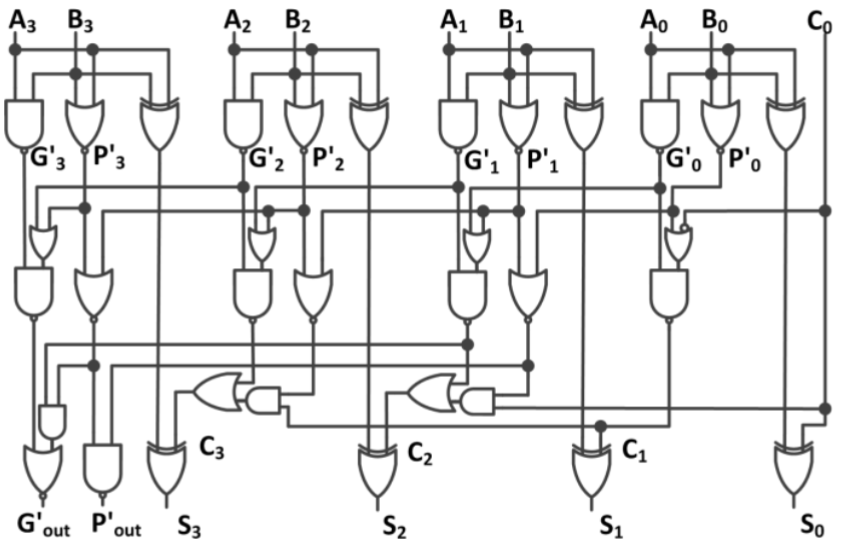
\includegraphics[width=1\linewidth]{Circuit_Diagram.png}
    \caption{4-bit Carry Look-Ahead Adder Design}
    \label{fig:cla}
    \end{figure}

\subsubsection{Propagate \& Generate Block}
This block includes three gates for each carry bit: One NOR gate for the Propagate signal, one NAND gates for the Generate signal and one XOR gate for the Sum signal.

\begin{figure}[H]
    \centering
    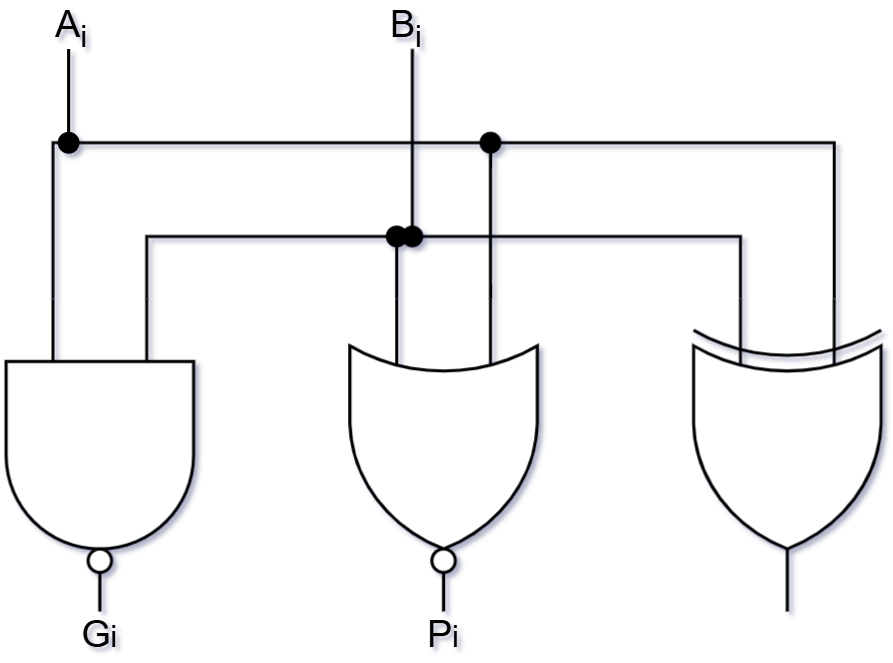
\includegraphics[width=0.5\linewidth]{propgencir.png}
    \caption{Propagate \& Generate Block}
    \label{fig:propagate_generate}
\end{figure}

Accoroding to the method of logical effort, the size of these gates is larger i.e. just double the proceedings gates of the intermediate block of CLA. So, the table below shows the sizing of gates in this block:

\begin{table}[H]
\centering
\caption{Sizing of Gates in Propagate \& Generate Block}
\begin{tabular}{|c|c|c|c|}
\hline
\rowcolor{cyan!10}
\textbf{Gate} & \textbf{Width ($W_N / W_P$) ($\mu m$)} & \textbf{Length ($\mu m$)} & \textbf{Number of Gates} \\ \hline
NOR          & 3.6 / 7.2                 & 0.18                  & 4                        \\ \hline
NAND         & 3.6 / 3.6                 & 0.18                  & 4                        \\ \hline
XOR          & 0.36 / 0.72               & 0.18                  & 4                        \\ \hline
\end{tabular}
\label{tab:propagate_generate}
\end{table} 

\subsubsection{Carry Look Ahead Block}
This block again further divided into two more subblocks namely intermediate block and AndOr block. The intermediate and the AndOr block includes three gates and two gates respectively for each carry bit. The intermediate block includes a NOR gate, NAND and OR gate and the AndOr block includes one AND gate and one OR gate.

\begin{figure}[H]
    \centering
    \includegraphics[width=0.9\linewidth]{clacir.png}
    \caption{Carry Look Ahead Block for Single Carry Bit}
    \label{fig:cla_block}
\end{figure}

The sizing of gates in the intermediate and AndOr block is done as per the method of logical effort. As a result, also mentioned in the previous block that this block sizing is half of the propagate \& generate block sizing. The OR gate is implemented using the NOR gate with an inverter at the output. Similarly for the AND gate, the NAND gate is used with an inverter at the output. The table below shows the sizing of gates in these blocks:

\begin{table}[H]
\centering
\caption{Sizing of Gates in Intermediate and AndOr Blocks}
\begin{tabular}{|c|c|c|c|}
\hline
\rowcolor{cyan!10}
\textbf{Block} & \textbf{Gate} & \textbf{Width ($W_N / W_P$) ($\mu m$)} & \textbf{Length ($\mu m$)} \\ \hline
\multirow{3}{*}{Intermediate} & NOR  & 0.9 / 1.8   & 0.18  \\ \cline{2-4} 
                              & NAND & 1.8 / 1.8   & 0.18  \\ \cline{2-4} 
                              & OR   & 0.9 / 1.8   & 0.18  \\ \hline
\multirow{2}{*}{AndOr}        & AND  & 1.8 / 1.8   & 0.18  \\ \cline{2-4}
                              & OR   & 0.9 / 1.8   & 0.18  \\ \hline 
Inverter                      & -    & 0.9 / 1.8   & 0.18  \\ \hline   
\end{tabular}
\label{tab:cla_block}
\end{table}

\subsubsection{Sum Block}
This block includes single XOR gate for the Sum signal which is implemented using Pass Transistor Logic. The sizing of this is set to be least possible just enough to drive the W-sized inverter and satisfy the DRC constraints because it is the last block in the design and don't have to drive any other block.

\begin{figure}[H]
    \centering
    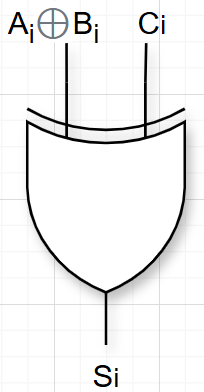
\includegraphics[width=0.2\linewidth]{sumcir.png}
    \caption{Sum Block}
    \label{fig:sum_block}
\end{figure}

\begin{table}[H]
\centering
\caption{Sizing of Gates in Sum Block}
\begin{tabular}{|c|c|c|c|}
\hline
\rowcolor{cyan!10}

\textbf{Gate} & \textbf{Width ($W_N / W_P$) ($\mu m$)} & \textbf{Length ($\mu m$)} & \textbf{Number of Gates} \\ \hline
XOR          & 0.36 / 0.72      & 0.18         & 6        \\ \hline
\end{tabular}
\label{tab:sum_block}
\end{table}

\subsubsection{D-Flip Flop}
It is implemented using the True Single Phase Clocked (TSPC) technology. It includes total no. of 12 transistors in CMOS logic style. The sizing of this is done by equating the resistances with the minimum W-sized inverter. There are two parts in the postive edge trigerred TSPC D-Flip Flop: Low-Level Latch and High-Level Latch.

\begin{figure}[H]
    \centering
    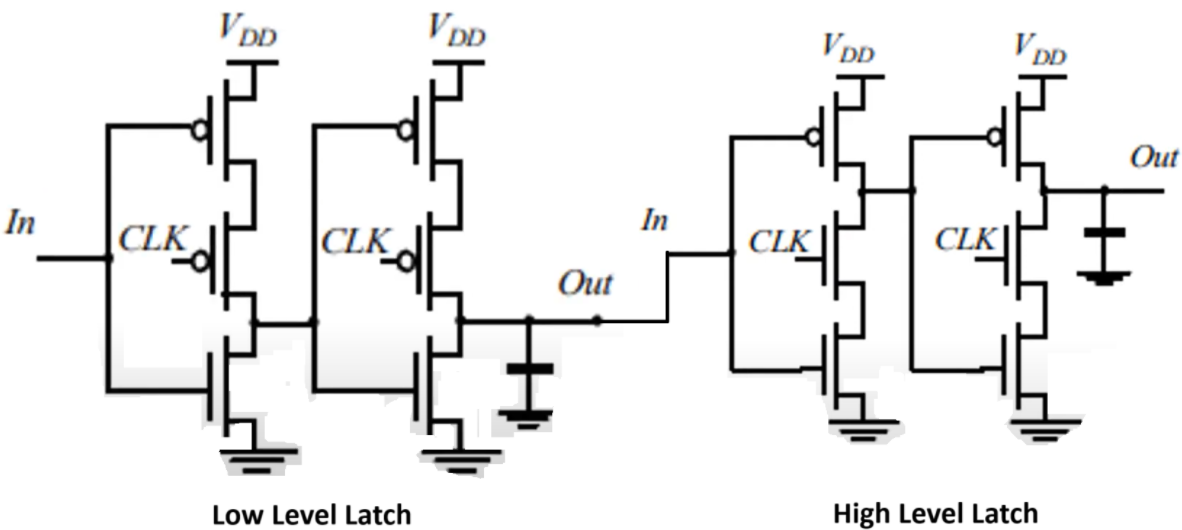
\includegraphics[width=1\linewidth]{TSPC.png}
    \caption{TSPC D-Flip Flop}
    \label{fig:dff}
\end{figure}

\begin{table}[H]
    \centering
    \caption{Sizing of Transistors in TSPC D-Flip Flop}
    \begin{tabular}{|c|c|c|c|}
    \hline
    \rowcolor{cyan!10}
    \textbf{Block} & \textbf{Transistor} & \textbf{Width ($\mu m$)} & \textbf{Length ($\mu m$)} \\ \hline
    \multirow{3}{*}{Low-Level Latch} & PMOS & 3.6 & 0.18 \\ \cline{2-4}
                                     & NMOS & 0.9 & 0.18 \\ \hline
    \multirow{3}{*}{High-Level Latch} & PMOS & 1.8 & 0.18 \\ \cline{2-4}
                                      & NMOS & 1.8 & 0.18 \\ \hline
    \end{tabular}
    \label{tab:dff_sizing}
\end{table}

\section{Delay Characteristics of D-Flip Flop (Prelayout)}
The TSPC D Flip-Flop was simulated using NGSPICE with a clock period of 2ns and input period of 4ns. Both clock and input signals were given sharp rise/fall times of 50ps to analyze the flip-flop's delay characteristics.

\subsection{Clock to Q Delay }
Upon simulating, we observe the following waveforms and terminal outputs:

\begin{figure}[H]
    \centering
    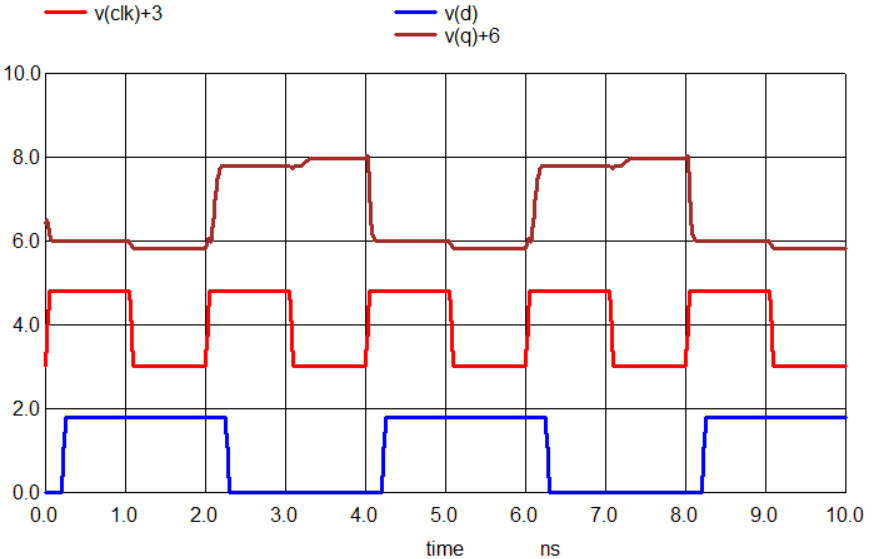
\includegraphics[width=1\linewidth]{dflipsimres.png}
    \caption{Waveforms Output of D-Flip Flop}
    \label{fig:dff_delay}
\end{figure}

\begin{figure}[H]
    \centering
    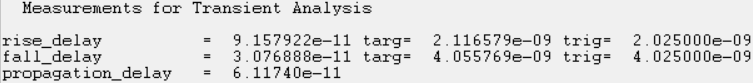
\includegraphics[width=1\linewidth]{dflipterm.png}
    \caption{Terminal Output for Delay}
    \label{fig:dff_power}
\end{figure}

The simulation gives the following timing parameters:
\begin{itemize}
    \item Rise Delay: 91.58ps - Time taken for the output to rise after the triggering clock edge
    \item Fall Delay: 30.77ps - Time taken for the output to fall after the triggering clock edge  
    \item Average Propagation Delay: 61.17ps - Mean of rise and fall delays
\end{itemize}

The asymmetry between rise and fall delays (ratio $\approx$ 3:1) can be attributed to:
\begin{itemize}
    \item Different sizing of PMOS/NMOS transistors in the low-level and high-level latches
    \item Inherent mobility difference between PMOS and NMOS devices
    \item Cascaded structure of the latches affecting signal propagation paths
\end{itemize}

\subsection{Setup Time}
Setup time ($t_{setup}$) is the minimum time before the active clock edge during which the data input (D) must remain stable. For TSPC D flip-flop, setup time is equal to the propagation delay of the Low-Level Latch because when clock is low, the Low-Level Latch is active and as it rises to high, the correct stable value of D must be present at the output of the Low-Level Latch for ensuring correct operation. This stable value of D appears at the output of the Low-Level Latch after the propagation delay of the Low-Level Latch.

\begin{figure}[H]
    \centering
    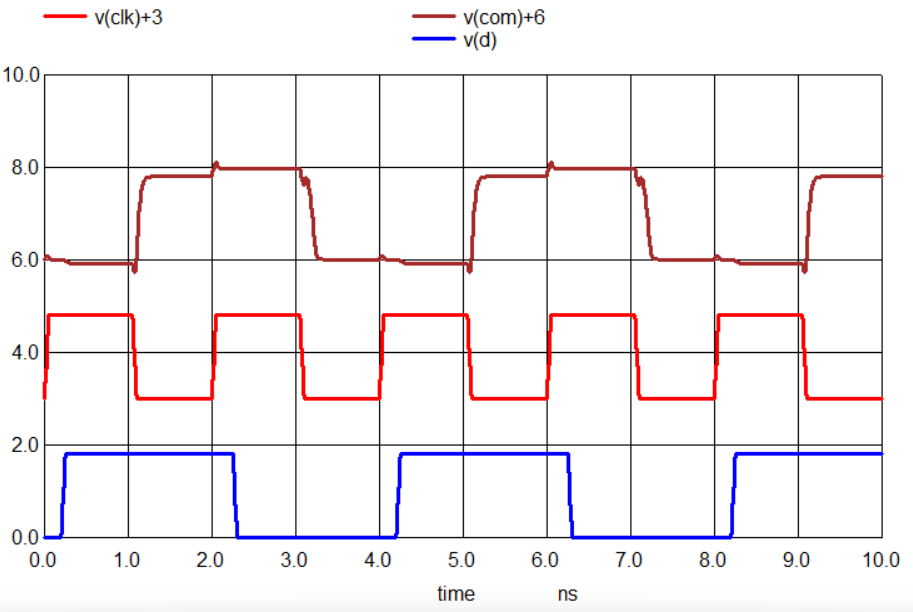
\includegraphics[width=1\linewidth]{dflipsetupsimres.png}
    \caption{Waveforms Output of Low-Level Latch}
    \label{fig:dff_setup}
\end{figure}

\begin{figure}[H]
    \centering
    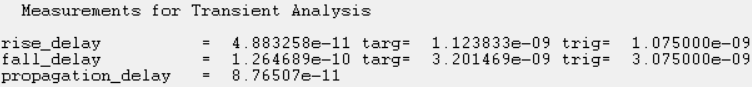
\includegraphics[width=1\linewidth]{dflipsetupterm.png}
    \caption{Terminal Output for Setup Time}
    \label{fig:dff_setup_term}
\end{figure}

\subsection{Hold Time}
Hold time ($t_{hold}$) is the minimum time after the active clock edge during which the data input must remain stable. For TSPC D flip-flop, hold time is zero because the High-Level Latch is active when the clock is high and the output of the High-Level Latch is not dependent on the input D when the clock is high. Therefore, the input D can change immediately after the active clock edge without affecting the output Q.


\begin{table}[H]
    \centering
    \caption{Timing Characteristics of TSPC D-Flip Flop}
    \begin{tabular}{|c|c|}
    \hline
    \rowcolor{cyan!10}
    \textbf{Parameter} & \textbf{Value (ps)} \\ \hline
    Rise Delay & 91.58 \\ \hline
    Fall Delay & 30.77 \\ \hline
    Propagation Delay & 61.17 \\ \hline
    Setup Time & 87.65  \\ \hline
    Hold Time & 0 \\ \hline
    \end{tabular}
    \label{tab:dff_timing}
    \end{table}

\section{Stick Diagram of Unique Gates}

\subsection{Inverter}
\begin{figure}[H]
    \centering
    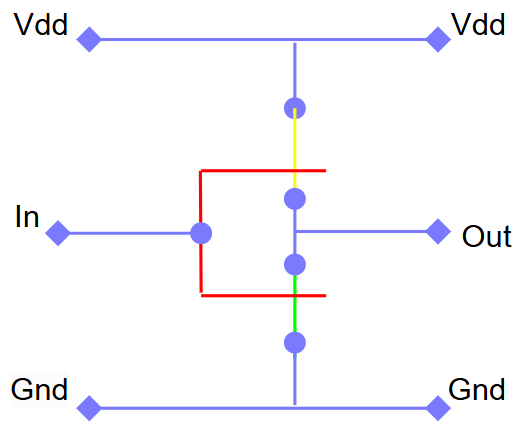
\includegraphics[width=0.5\linewidth]{stickinv.png}
    \caption{Inverter Stick Diagram}
    \label{fig:inverter}
\end{figure}

\subsection{NOR Gate}
\begin{figure}[H]
    \centering
    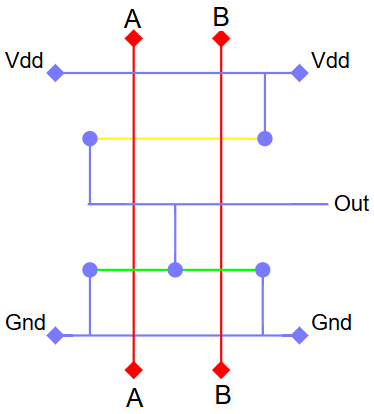
\includegraphics[width=0.5\linewidth]{sticknor.png}
    \caption{NOR Gate Stick Diagram}
    \label{fig:nor}
\end{figure}


\subsection{NAND Gate}
\begin{figure}[H]
    \centering
    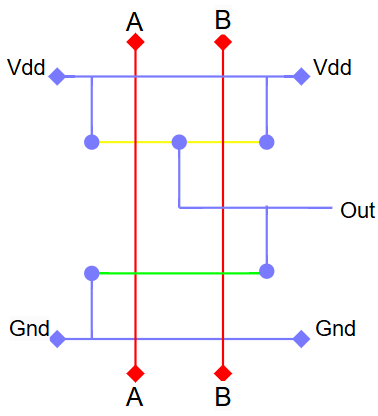
\includegraphics[width=0.5\linewidth]{sticknand.png}
    \caption{NAND Gate Stick Diagram}
    \label{fig:nand}
\end{figure}

\subsection{XOR Gate}
\begin{figure}[H]
    \centering
    \includegraphics[width=0.5\linewidth]{example-image-a.png}
    \caption{XOR Gate Stick Diagram}
    \label{fig:xor}
\end{figure}


% \section{Prelayout Full Circuit Analysis}

\section{Prelayout Simulation Results \& Analysis of CLA}
The 4-bit Carry Look-ahead Adder was simulated using NGSPICE with the following test conditions:

\subsection{Verification of functionality}
\subsubsection{Input Specifications}
\begin{itemize}
    \item Supply Voltage (VDD): 1.8V
    \item Input A (4-bit):
    \begin{itemize}
        \item A0: Pulse starting at 10ns, Period = 40ns
        \item A1: Pulse starting at 15ns, Period = 50ns
        \item A2: Pulse starting at 20ns, Period = 60ns
        \item A3: Pulse starting at 25ns, Period = 70ns
        \item Rise/Fall times: 50ps
    \end{itemize}
    
    \item Input B (4-bit):
    \begin{itemize}
        \item B0: Pulse starting at 12ns, Period = 44ns
        \item B1: Pulse starting at 18ns, Period = 56ns
        \item B2: Pulse starting at 24ns, Period = 68ns
        \item B3: Pulse starting at 30ns, Period = 80ns
        \item Rise/Fall times: 50ps
    \end{itemize}
    \item Carry Input (Cin): Pulse starting at 36ns, Period = 88ns
    \item Clock (CLK): Period = 8ns
\end{itemize}

\subsubsection{Output Analysis}
The simulation produces the following outputs:
\begin{itemize}
    \item Sum outputs (S0-S3): Generated through XOR combinations of inputs and internal carries
    \item Final Carry (C4): Represents the overflow from the 4-bit addition
\end{itemize}

\begin{figure}[H]
    \centering
    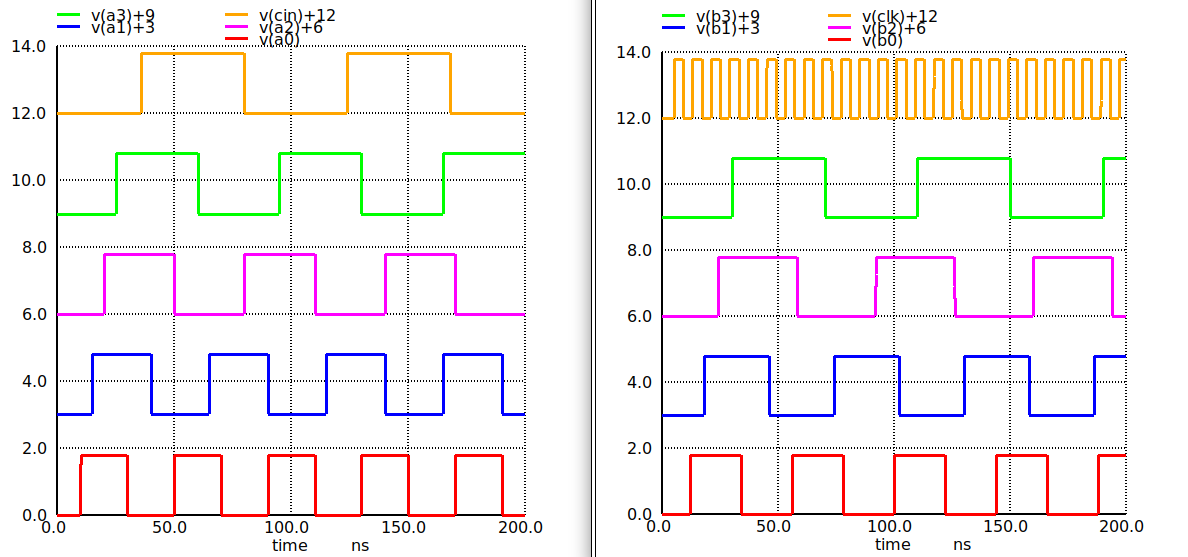
\includegraphics[width=1\linewidth]{claprengspi.png}
    \caption{Input Waveform}
    \label{fig:cla_waveform}
\end{figure}

Above plots show the input waveforms given to the 4-bit CLA. The left plot shows the A bits along with $C_{in}$ and right one shows the B bits along with the clock.

\begin{figure}[H]
    \centering
    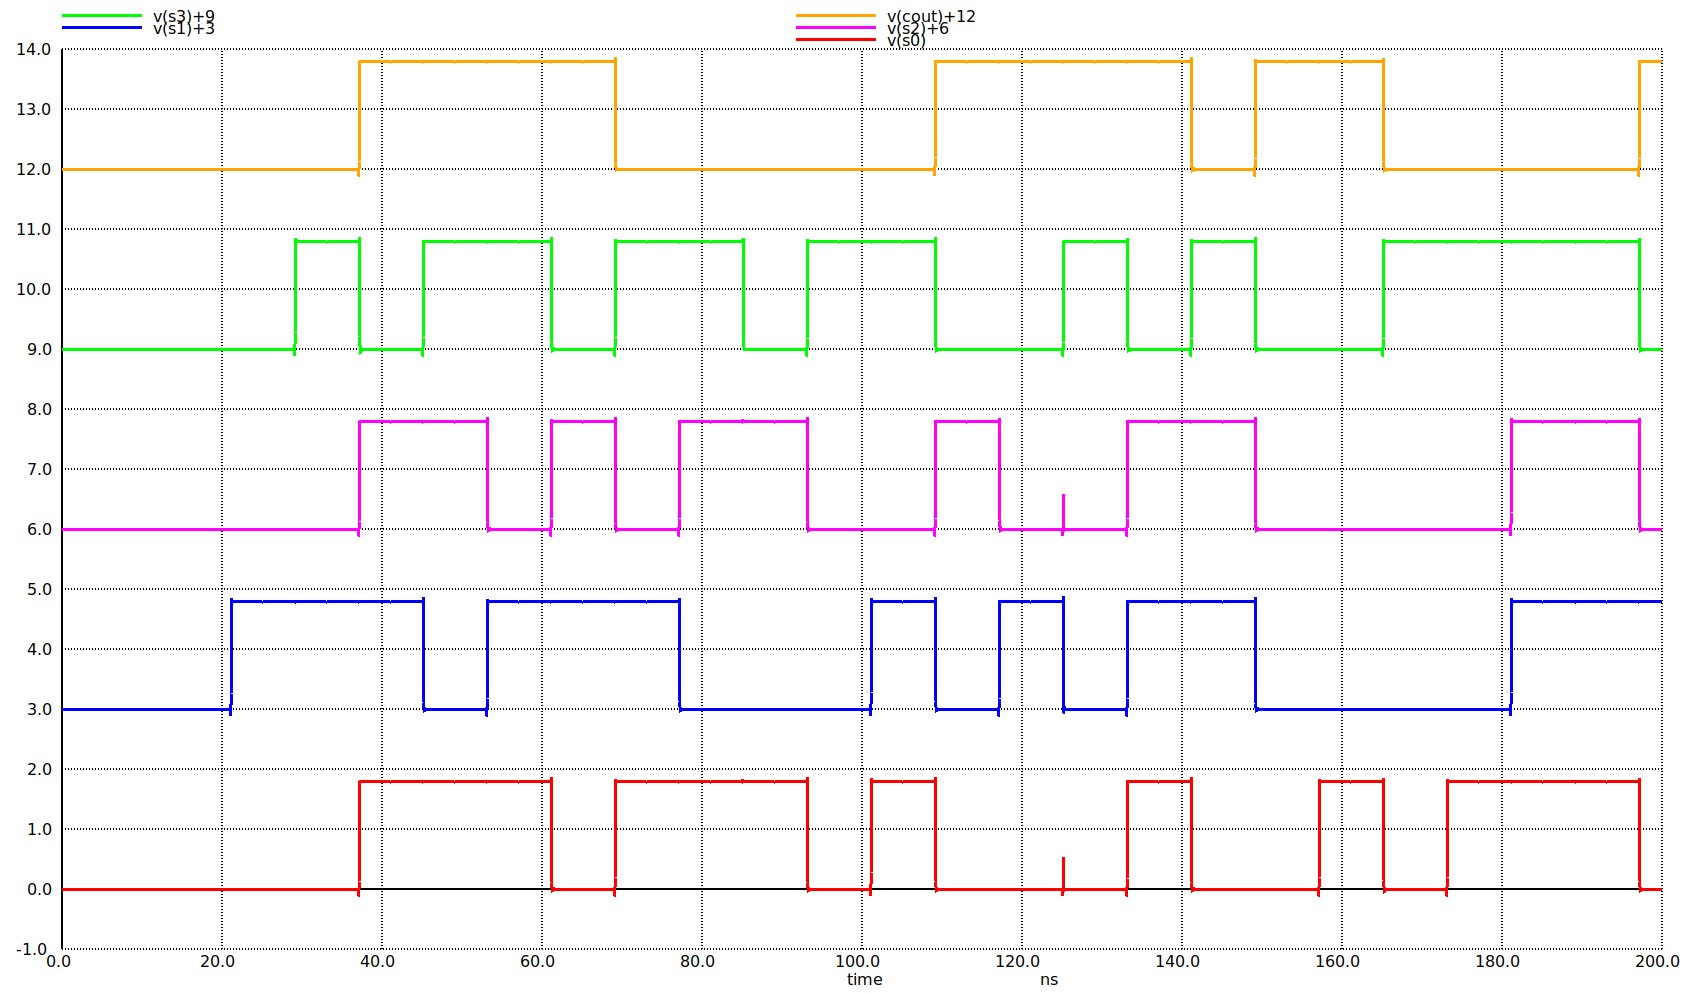
\includegraphics[width=1\linewidth]{claprengspi2.png}
    \caption{Output Waveform}
    \label{fig:cla_terminal}
\end{figure}

Above plot shows the output waveforms which includes the four Sum bits and the final Carry bit.

The waveforms demonstrate correct operation of the CLA with proper carry propagation and sum generation across all bit positions. The progressive delays in input signals help verify the adder's functionality under varying timing conditions.

\subsection{Worst Case Delay of CLA Adder Block}
Worst case delay is the maximum time taken for the output to stabilize after the input changes. This happens in the path which has highest resistance or very large number of gates. In the 4-bit CLA design proposed above, the worst case delay is observed in the carry propagation path from  $B_0$ through C3 to S3 because it is the longest path with total 9 gates in midway. 
For considering the worst case delay, the S3 bit must change when B0 bit changes. So, here we take the input signals as follows:
\begin{itemize}
    \item $A_0 = A_1 = A_2 = A_3 = 0, B_1 = B_2 = 1, B_3 = 0$
    \item $B_0$: Pulse starting at 25ns, Period = 70ns
    \item $C_{in}$ = 1
    \item Clock (CLK): Pulse starting at 0ns, Period = 8ns
\end{itemize}

With the above inputs, we get the simulation results for the worst case delay as follows:
\begin{figure}[H]
    \centering
    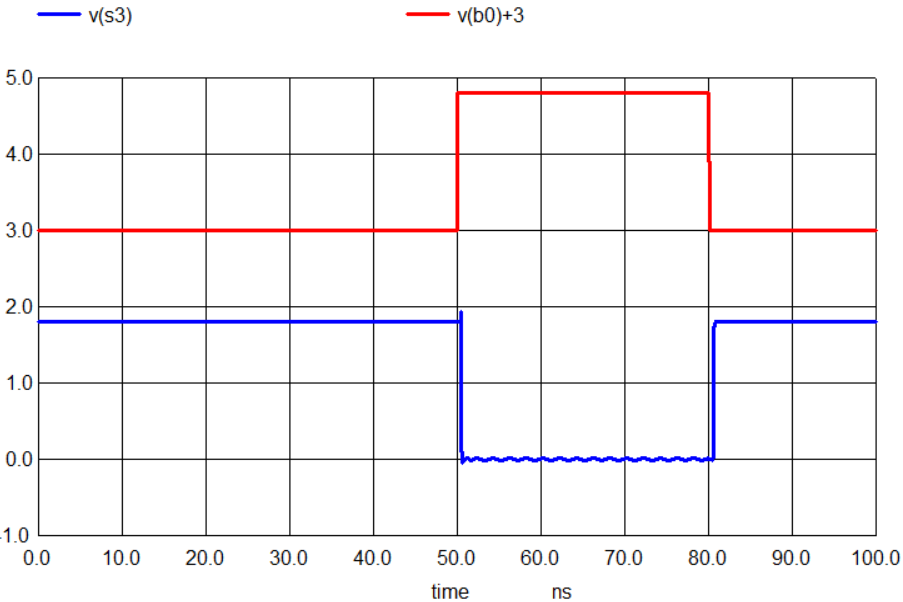
\includegraphics[width=1\linewidth]{clapreworst.png}
    \caption{WaveForms for the Worst Case Delay}
    \label{fig:worst_case_delay}
\end{figure}

\begin{figure}[H]
    \centering
    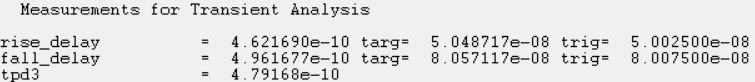
\includegraphics[width=1\linewidth]{clapreworstterm.png}
    \caption{Worst Case Delay Terminal Output}
    \label{fig:worst_case_delay}
\end{figure}

The simulation results show that the worst case delay for the 4-bit CLA design is 479.16ps. This delay is observed in the carry propagation path from $B_0$ through C3 to S3.

\subsection{Maximum Clock Speed}

\subsubsection{Theoritical Calculation}
The maximum clock speed of the 4-bit CLA design can be calculated using the following inequality:
    \begin{align}
        t_{CQ_1} + t_{pd} + t_{su} \leq T_{clk} \\
        f_{max} = \frac{1}{t_{CQ_1} + t_{pd} + t_{su}}
    \end{align}
    where $t_{CQ_1}$ is the clock-to-Q delay of the first flip-flop, $t_{pd}$ is the worst-case propagation delay of the CLA adder block, and $t_{su}$ is the setup time of the flip-flop.

    Given the values we calculated earlier:
    \begin{itemize}
        \item $t_{CQ_1} = 61.17 \text{ ps}$
        \item $t_{pd} = 479.16 \text{ ps}$
        \item $t_{su} = 87.65 \text{ ps}$
    \end{itemize}

    The maximum clock frequency is:
    \begin{equation}
        f_{max} = \frac{1}{61.17 \text{ ps} + 479.16 \text{ ps} + 87.65 \text{ ps}} \approx 1.59 \text{ GHz}
    \end{equation}

\subsubsection{Found using Simulation}
Using the Ngspice Simulation, I found that the maximum clock frequency of the 4-bit CLA design is 1.04 GHz which is less than the theoritical value. This difference can be attributed to the following factors:
\begin{itemize}
    \item Parasitic Capacitances: The simulation does not consider the parasitic capacitances which can affect the delay and hence the maximum clock frequency.
    \item Wire Delays: The simulation does not consider the wire delays which can affect the delay and hence the maximum clock frequency.
\end{itemize}

\section{Delay Characteristics of D-Flip Flop (Postlayout)}
The TSPC D Flip-Flop was simulated using NGSPICE with a clock period of 2ns and input period of 4ns. Both clock and input signals were given sharp rise/fall times of 50ps to analyze the flip-flop's delay characteristics.

\subsection{Clock to Q Delay }
Upon simulating, we observe the following waveforms and terminal outputs:

% \begin{figure}[H]
%     \centering
%     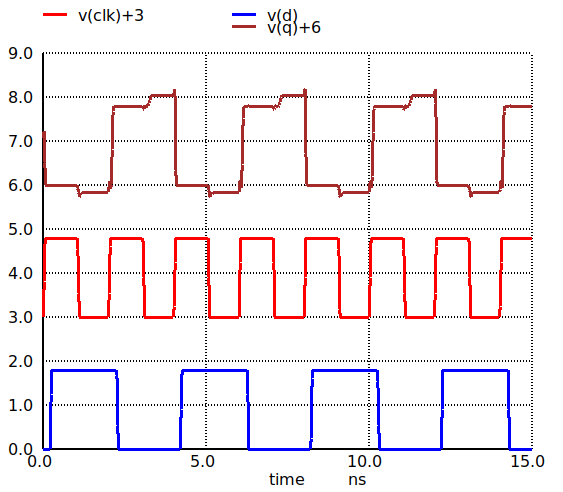
\includegraphics[width=1\linewidth]{dflippostsetup.png}
%     \caption{Waveforms Output of D-Flip Flop}
%     \label{fig:dff_delay}
% \end{figure}

% \begin{figure}[H]
%     \centering
%     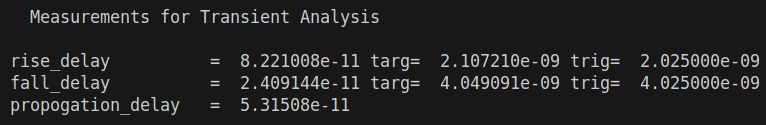
\includegraphics[width=1\linewidth]{dflippostsetupterm.png}
%     \caption{Terminal Output for Delay}
%     \label{fig:dff_power}
% \end{figure}

The simulation gives the following timing parameters:
\begin{itemize}
    \item Rise Delay: 92.21ps - Time taken for the output to rise after the triggering clock edge
    \item Fall Delay: 24.09ps - Time taken for the output to fall after the triggering clock edge  
    \item Average Propagation Delay: 53.15ps - Mean of rise and fall delays
    \item Setup Time: 87.65ps - Minimum time before the active clock edge during which the data input must remain stable
    \item Hold Time: 0ps - Minimum time after the active clock edge during which the data input must remain stable
\end{itemize}


\section{Post-Layout Simulation Results \& Analysis of CLA}
The 4-bit CLA desgign layout was implemented in 180nm technology in magic as shown in the figure below. The layout was then extracted and simulated using NGSPICE with the same test conditions as the pre-layout simulation.

\begin{figure*}[h]
    \centering
    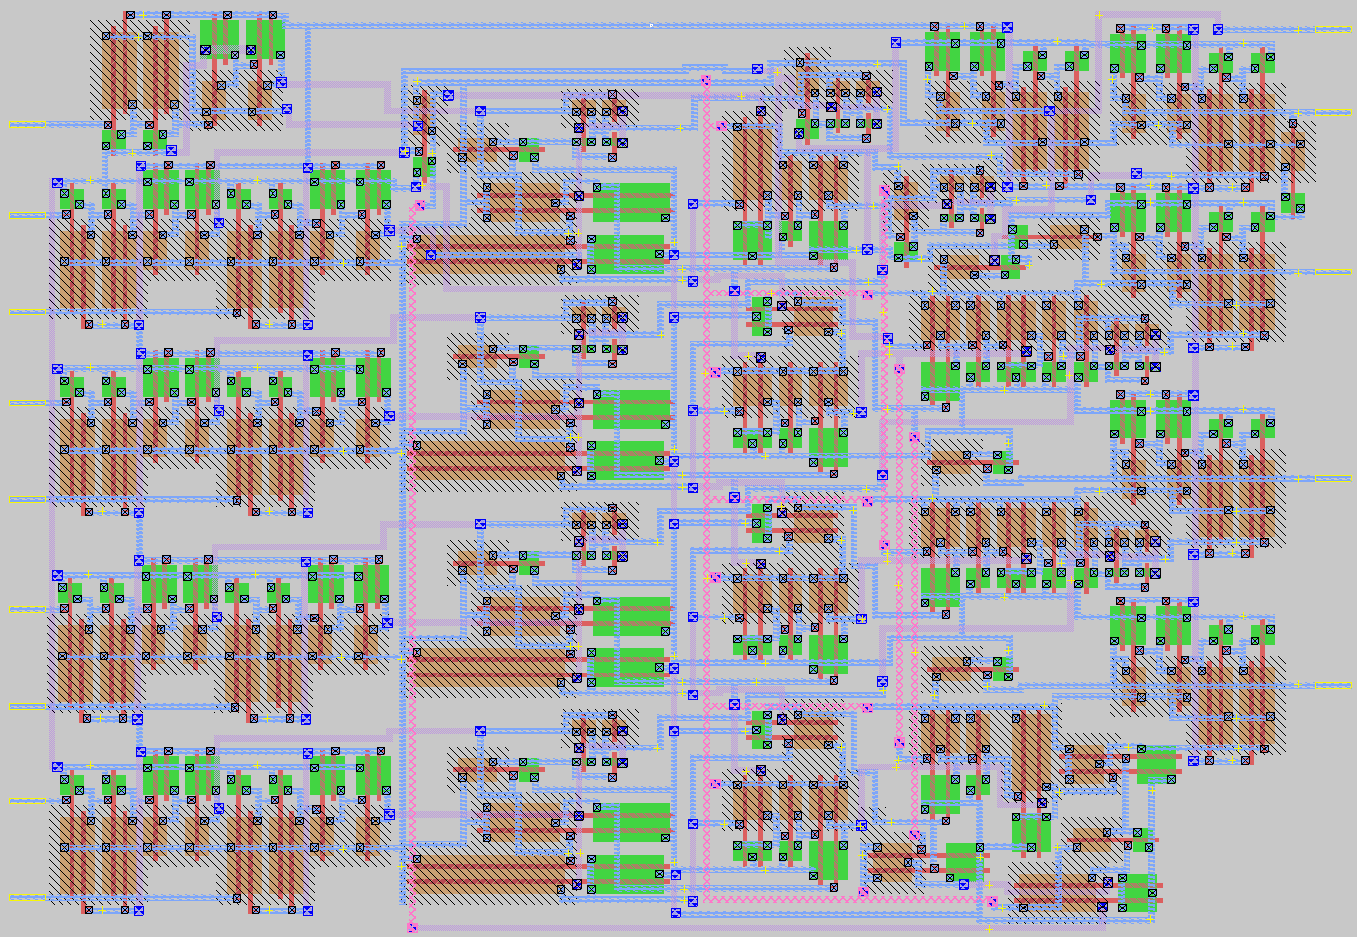
\includegraphics[width=1\linewidth]{clapostmag.png}
    \caption{Magic Layout of 4-bit CLA Design}
    \label{fig:layout}
\end{figure*}

\subsection{Verification of functionality}
The input and output specifications are same as mentioned previously in the prelayout simulation. 
The post-layout simulation produces the following outputs:

\begin{figure}[H]
    \centering
    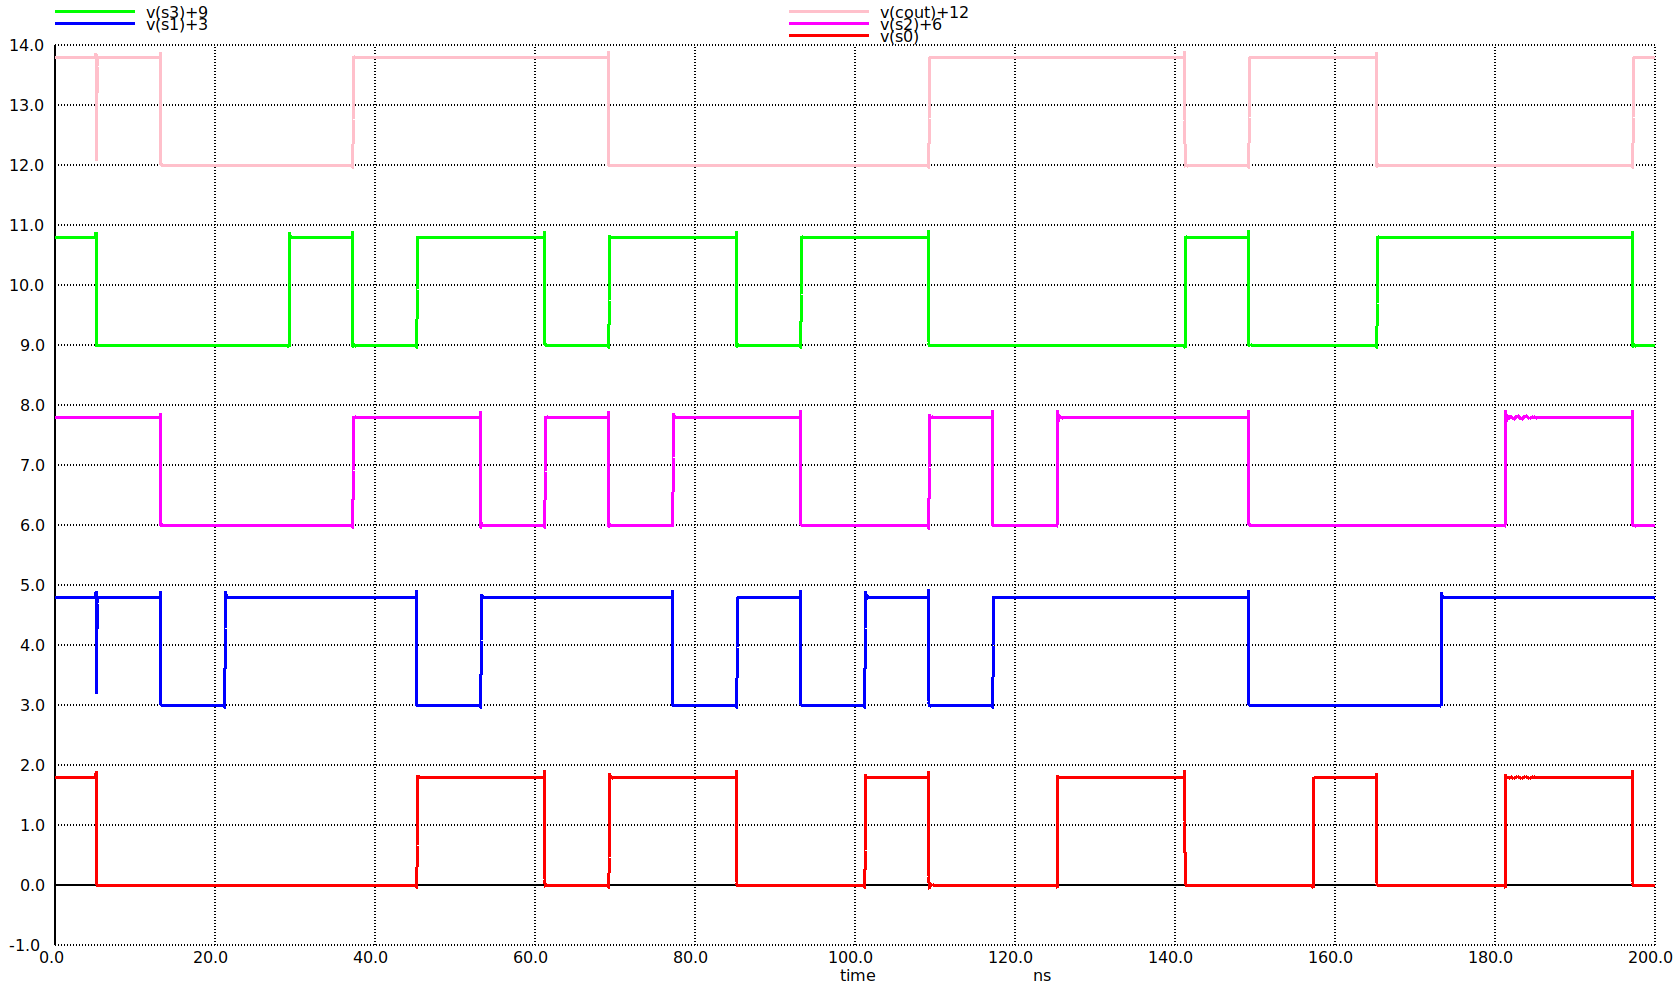
\includegraphics[width=1\linewidth]{clapostngspi2.png}
    \caption{Input Waveform}
    \label{fig:cla_waveform}
\end{figure}

The intial outputs are different from the prelayout simulation because of the initial conditions of the flip-flops. After few clock cycles, the outputs stabilize and matches exactly with the prelayout simulation hence the correct operation of the CLA is verified.

\subsection{Worst Case Delay of CLA Adder Block}
The worst case delay of the post-layout 4-bit CLA design is calculated using the same inputs as in the pre-layout simulation. The simulation results for the worst case delay are as follows:

\begin{figure}[H]
    \centering
    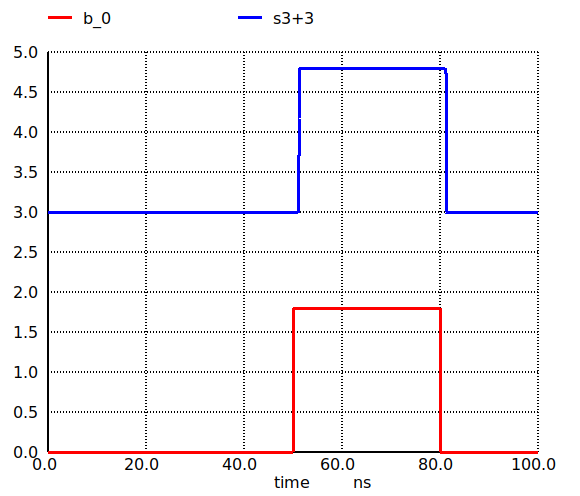
\includegraphics[width=1\linewidth]{clapostworst.png}
    \caption{WaveForms for the Worst Case Delay}
    \label{fig:worst_case_delay}
\end{figure}

\begin{figure}[H]
    \centering
    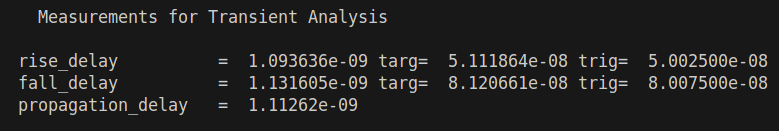
\includegraphics[width=1\linewidth]{clapostworstterm.png}
    \caption{Worst Case Delay Terminal Output}
    \label{fig:worst_case_delay}
\end{figure}

The simulation results show that the worst case delay for the post-layout 4-bit CLA design is 1112.62ps. This delay is observed in the carry propagation path from $B_0$ through C3 to S3.

\subsection{Maximum Clock Speed}
The maximum clock speed of the post-layout 4-bit CLA design is calculated using the same method as in the pre-layout simulation. Given the values we calculated earlier:
\begin{itemize}
    \item $t_{CQ_1} = 61.17 \text{ ps}$
    \item $t_{pd} = 1112.62 \text{ ps}$
    \item $t_{su} = 87.65 \text{ ps}$
\end{itemize}

The maximum clock frequency is:
\begin{equation}
    f_{max} = \frac{1}{61.17 \text{ ps} + 1112.62 \text{ ps} + 87.65 \text{ ps}} \approx 0.78 \text{ GHz}
\end{equation}

% comparison table between pre and post layout simulation results
\begin{table}[H]
    \centering
    \caption{Comparison of Pre and Post Layout Simulation Results}
    \begin{tabular}{|c|c|c|}
    \hline
    \rowcolor{cyan!10}
    \textbf{Parameter} & \textbf{Pre-Layout} & \textbf{Post-Layout} \\ \hline
    Worst Case Delay (ps) & 479.16 & 1112.62 \\ \hline
    Maximum Clock Frequency (GHz) & 1.59 & 0.78 \\ \hline
    \end{tabular}
    \label{tab:comparison}
\end{table}

\section{Floor Plan for Complete Circuit Layout}

\begin{figure*}[h]
    \centering
    \includegraphics[width=1\linewidth]{example-image-a.png}
    \caption{Floor Plan for Complete Circuit Layout}
    \label{fig:floorplan}
\end{figure*}

\section{Verilog HDL Simulation Results}

\begin{figure*}[h]
    \centering
    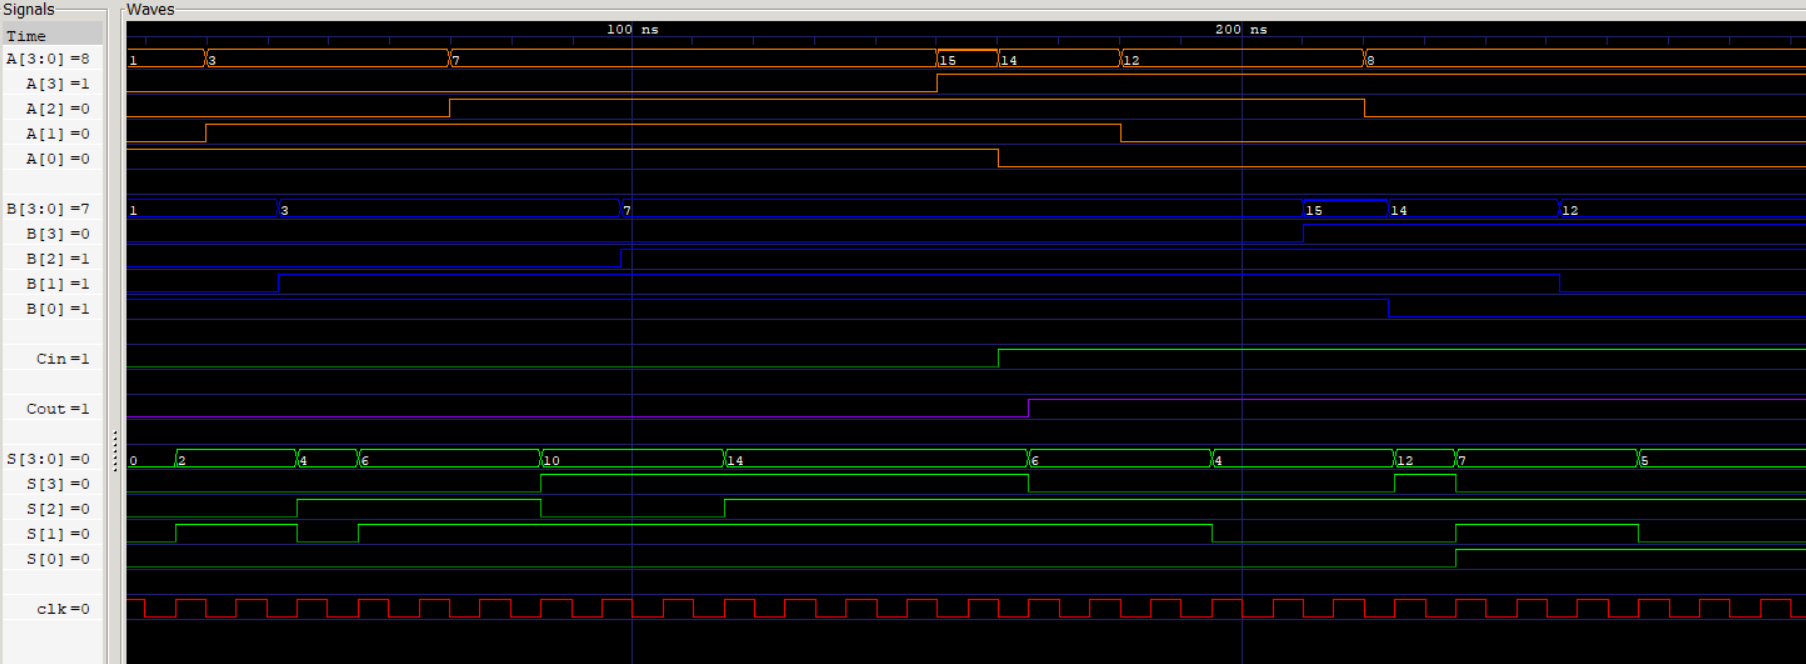
\includegraphics[width=1\linewidth]{veriloggtk.png}
    \caption{Verilog HDL Simulation Waveforms}
    \label{fig:verilog_waveform}
\end{figure*}

\section{Implementaion on FPGA board and oscilloscope}

% \begin{figure*}[h]
%     \centering
%     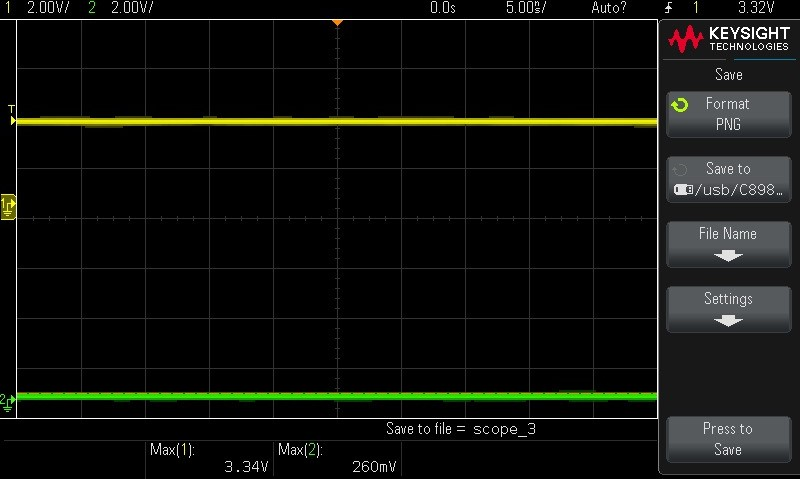
\includegraphics[width=1\linewidth]{oscillo1.png}
%     \caption{FPGA Implementation of 4-bit CLA}
%     \label{fig:fpga}
% \end{figure*}

% \begin{figure*}[h]
%     \centering
%     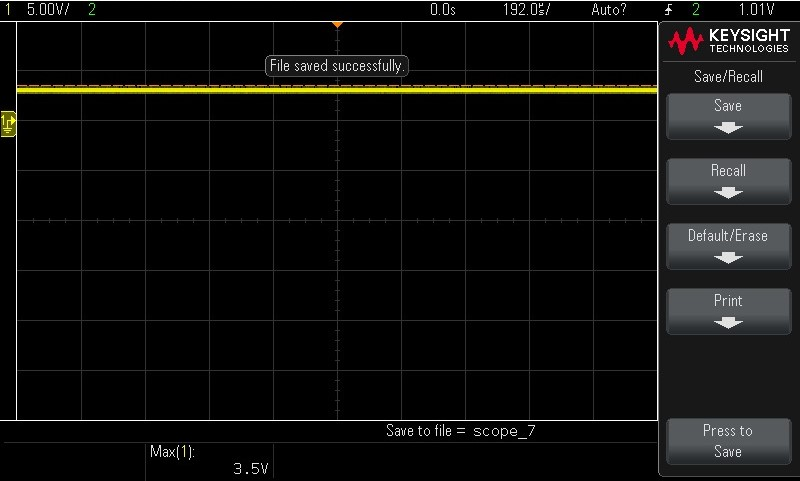
\includegraphics[width=1\linewidth]{oscillo2.png}
%     \caption{Oscilloscope Output of 4-bit CLA}
%     \label{fig:oscilloscope}
% \end{figure*}

% \begin{figure*}[h]
%     \centering
%     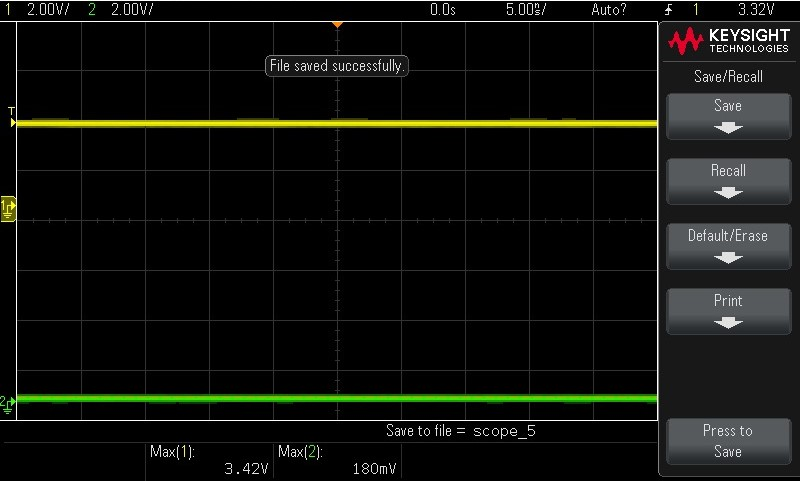
\includegraphics[width=1\linewidth]{oscillo3.png}
%     \caption{Oscilloscope Output of 4-bit CLA}
%     \label{fig:oscilloscope}
% \end{figure*}


\begin{table}[htbp]
\caption{Table Type Styles}
\begin{center}
\begin{tabular}{|c|c|c|c|}
\hline
\textbf{Table}&\multicolumn{3}{|c|}{\textbf{Table Column Head}} \\
\cline{2-4} 
\textbf{Head} & \textbf{\textit{Table column subhead}}& \textbf{\textit{Subhead}}& \textbf{\textit{Subhead}} \\
\hline
copy& More table copy$^{\mathrm{a}}$& &  \\
\hline
\multicolumn{4}{l}{$^{\mathrm{a}}$Sample of a Table footnote.}
\end{tabular}
\label{tab1}
\end{center}
\end{table}

\section*{References}

Please number citations consecutively within brackets \cite{b1}. The 
sentence punctuation follows the bracket \cite{b2}. Refer simply to the reference 
number, as in \cite{b3}---do not use ``Ref. \cite{b3}'' or ``reference \cite{b3}'' except at 
the beginning of a sentence: ``Reference \cite{b3} was the first $\ldots$''

Number footnotes separately in superscripts. Place the actual footnote at 
the bottom of the column in which it was cited. Do not put footnotes in the 
abstract or reference list. Use letters for table footnotes.

Unless there are six authors or more give all authors' names; do not use 
``et al.''. Papers that have not been published, even if they have been 
submitted for publication, should be cited as ``unpublished'' \cite{b4}. Papers 
that have been accepted for publication should be cited as ``in press'' \cite{b5}. 
Capitalize only the first word in a paper title, except for proper nouns and 
element symbols.

For papers published in translation journals, please give the English 
citation first, followed by the original foreign-language citation \cite{b6}.

\begin{thebibliography}{00}
\bibitem{b1} G. Eason, B. Noble, and I. N. Sneddon, ``On certain integrals of Lipschitz-Hankel type involving products of Bessel functions,'' Phil. Trans. Roy. Soc. London, vol. A247, pp. 529--551, April 1955.
\bibitem{b2} J. Clerk Maxwell, A Treatise on Electricity and Magnetism, 3rd ed., vol. 2. Oxford: Clarendon, 1892, pp.68--73.
\bibitem{b3} I. S. Jacobs and C. P. Bean, ``Fine particles, thin films and exchange anisotropy,'' in Magnetism, vol. III, G. T. Rado and H. Suhl, Eds. New York: Academic, 1963, pp. 271--350.
\bibitem{b4} K. Elissa, ``Title of paper if known,'' unpublished.
\bibitem{b5} R. Nicole, ``Title of paper with only first word capitalized,'' J. Name Stand. Abbrev., in press.
\bibitem{b6} Y. Yorozu, M. Hirano, K. Oka, and Y. Tagawa, ``Electron spectroscopy studies on magneto-optical media and plastic substrate interface,'' IEEE Transl. J. Magn. Japan, vol. 2, pp. 740--741, August 1987 [Digests 9th Annual Conf. Magnetics Japan, p. 301, 1982].
\bibitem{b7} M. Young, The Technical Writer's Handbook. Mill Valley, CA: University Science, 1989.
\end{thebibliography}
\vspace{12pt}
\color{red}
IEEE conference templates contain guidance text for composing and formatting conference papers. Please ensure that all template text is removed from your conference paper prior to submission to the conference. Failure to remove the template text from your paper may result in your paper not being published.

\end{document}
